% ------------------------------------------------------------------------
%%%%% Start of preamble %%%%%
% ------------------------------------------------------------------------

%%%%---------What kind of document  and what size--------------------------------------
\documentclass[12pt]{article}

%%%MY: Other possible document: article, report, amsart, thesis, book,etc.


%%%%---------Packages to load which give you useful commands---------------------------------
\usepackage{graphicx} %to include pictures and figures
\usepackage{amssymb, amsmath, amsthm} %to include standard Americam Mathematical Society math symbols and fonts
\usepackage{fontenc} %to be able to inlude more font
\usepackage{amscd,latexsym,amsfonts,amstext,amsbsy} %more AMS fonts and options
\usepackage{euscript} %for european script
\usepackage{enumerate} %for automatic enumeration of equations, items, etc.
\usepackage{color}  %to change the color of a text.
\usepackage{physics}
\usepackage[latin1]{inputenc}
\usepackage{tikz}
\usepackage{mathrsfs}
\usetikzlibrary{shapes,arrows}


%%%%---------Sets the margins--------------------------------------------------------------
%As example, the margins are manually chosen below.  You can change the margins if needed.
%%%In particular: Use default margins first (just insert % the the start of each of
%the lines below for LaTex to disregard the options, ---------------------

\textwidth = 16 cm
\textheight = 24 cm
\oddsidemargin = 0.0 cm
\evensidemargin = 0.0 cm
\topmargin = -2 cm
%\headheight = 0.0 in
%\headsep = 0.0 in
\parskip = 0.2in
\parindent = 0.0in

%%%%------------MY: sets up doublespacing: use 2  inside the {} below---------------------------------
%This allows me to include feedback between the lines.
%For singlespace  just use % to disregard the command or use 1 instead.
%\renewcommand{\baselinestretch}{2}


%%%---------------MY: New theorem type environments-------------------------------
 \newtheorem{theorem}{Theorem}
  \newtheorem{problem}[theorem]{Problem}
   \newtheorem{exercise}[theorem]{Exercise}
 \newtheorem{corollary}[theorem]{Corollary}
 \newtheorem{lemma}[theorem]{Lemma}
 \newtheorem{proposition}[theorem]{Proposition}
 \newtheorem{proporties}[theorem]{Proporties}
 \newtheorem{definition}[theorem]{Definition}
  \newtheorem{definitions}[theorem]{Definitions}
  \newtheorem{example}[theorem]{Example}
 \newtheorem{remark}[theorem]{Remark}
 


\begin{document}
%%%%%%This declares that your document starts here

January 13, 2018 \\
Heroin Model 


S=susceptibles\\
P=prescribed opioid users,
A=addicted to opioids, 
H=heroin users/addicted,
R=treatment/rehabilitation 
$S(0)=S_{0}$, $P(0)=P_{0}$, $A(0)=A_{0}$, $H(0)=H_{0}$, $R(0)=R_{0}$ \\
Assume $H_{0}>0$, $\mu_{H} > \mu_{A}$ and $\theta_{1} > \theta_{2}, \theta_{3}$ 
\[\dv{S}{t} = -\alpha S - \beta (1- \xi) SA  -\beta \xi SP- \theta_{1} SH +\epsilon P +\delta R +\mu (P+R) + (\mu+\mu_{A})A + (\mu+\mu_{H}) H \quad\]
\[\dv{P}{t} = \alpha S - \epsilon P  - \gamma P - \theta_{2}PH- \mu P    \quad\]
\[\dv{A}{t} = \gamma P + \sigma_{A} R +\beta (1- \xi) SA  +\beta \xi SP -\zeta A - \theta_{3}AH-(\mu + \mu_{A})A   \quad\]
\[\dv{H}{t} = \theta_{1}SH+\theta_{2}PH+\theta_{3}AH + \sigma_{H}R-\nu H-(\mu+\mu_{H})H  \quad\]
\[\dv{R}{t} = \zeta A +\nu H -\delta R -\sigma_{A}R-\sigma_{H}R -\mu R\quad\]


The following is a brief description of each parameter in the system: \\
$\alpha$: the rate at which people are prescribed opioids \\
$\beta$ : total probability of becoming addicted to opioids other than by prescription \\
$\beta(1-\xi)$: proportion of which the non-prescribed, susceptible population becomes addicted to opioids by black market drugs and other addicts \\
$\beta \xi$ : proportion of which the non-prescribed, susceptible population obtains extra prescription opioids and becomes addicted  \\
$\theta_1$: rate at which the non-prescribed, susceptible population becomes addicted to heroin by black market drugs and other addicts  \\
$\epsilon$: rate at which people come back to the susceptible class after being prescribed opioids (i.e. not addicted)\\
$\delta$: rate at which people come back to the susceptible class after successfully finishing treatment \\
$\mu$: natural death rate \\
$\mu_A$: enhanced death rate for opioid addicts (overdose rate which results in death) \\
$\mu_H$: enhanced death rate for heroin addicts (overdose rate which results in death) \\
$\gamma$: rate at which prescribed opioid users become addicted \\
$\theta_2$: rate at which opioid prescribed user population becomes addicted to heroin \\
$\sigma_A$: rate at which people relapse from treatment into the opioid addicted class \\
$\zeta$: rate at which addicted opioid users enter treatment/rehabilitation \\
$\theta_3$: rate at which the opioid addicted population becomes addicted to heroin \\
$\sigma_H$: rate at which people relapse from treatment into the heroin addicted class \\
$\nu$: rate at which heroin users enter treatment/rehabilitation \\ \\



\begin{figure}
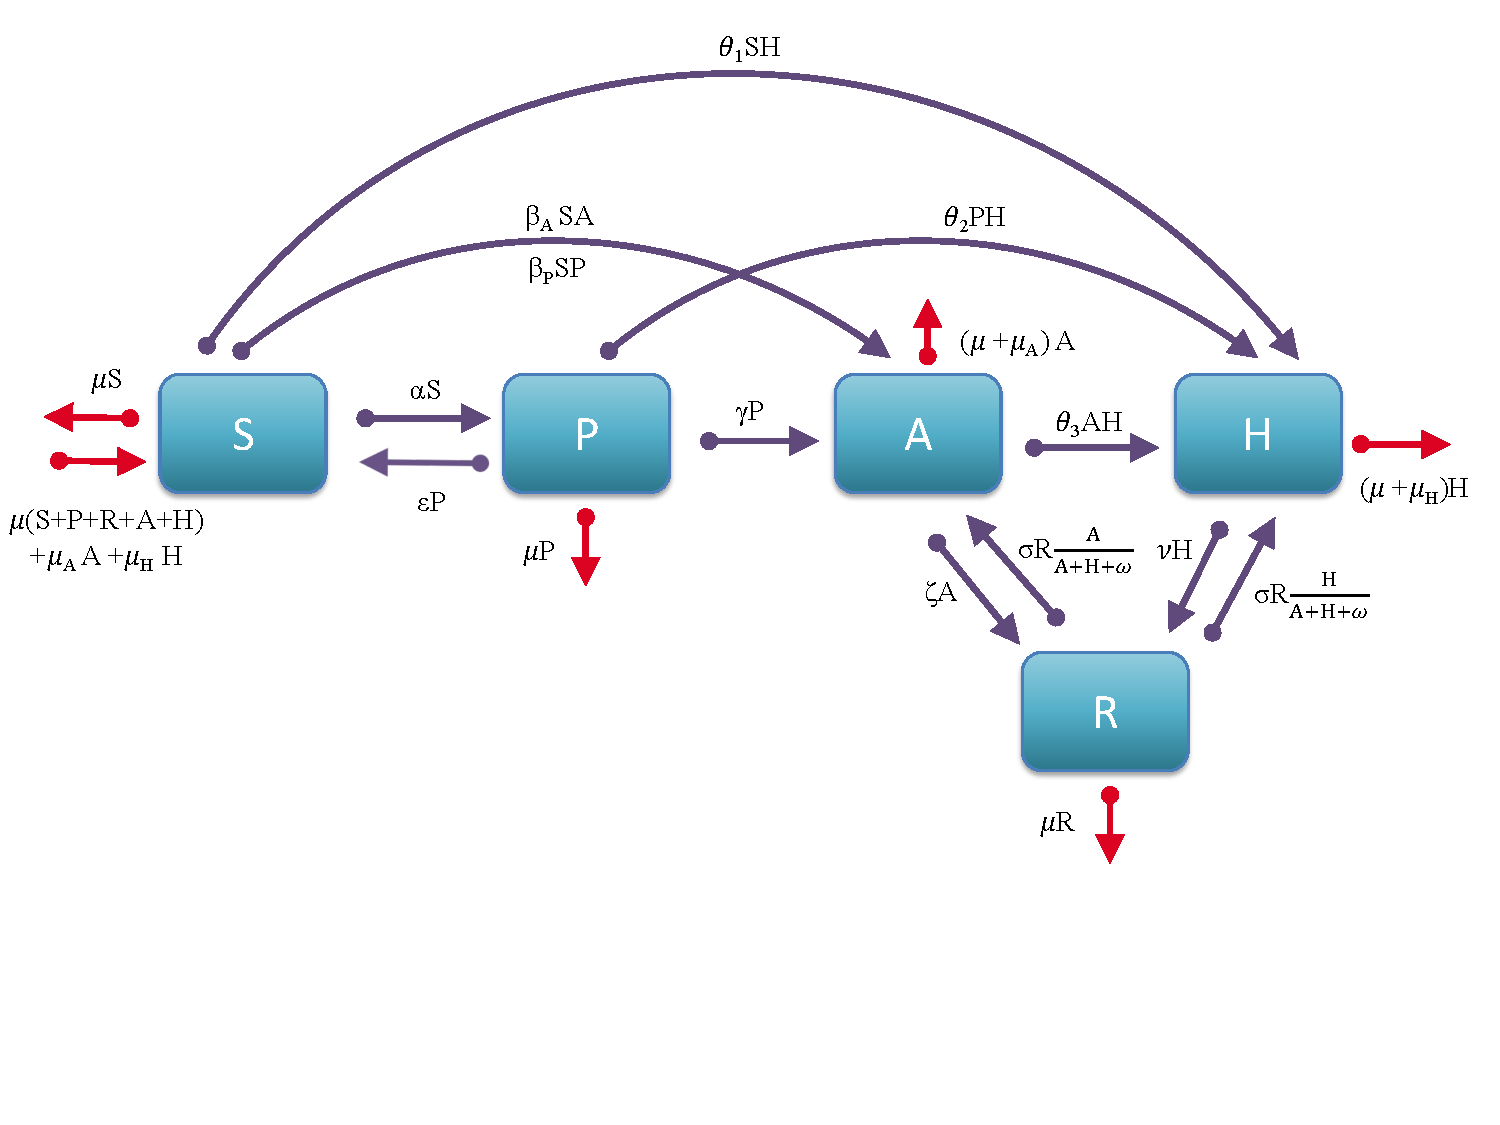
\includegraphics[scale=0.66]{heroin_schematic.pdf}
\end{figure}


To find the addiction-free equilibrium (AFE), we set Eqs. (FILL IN) equal to zero and require that $A=H=R=0$. We are left with the system \\

\[0=-\alpha S^* -\beta \xi S^* P^* + \epsilon P^* +\mu P^* \quad\]
\[0=\alpha S^* - \epsilon P^* -\gamma P^* - \mu P^* \quad\]
\[0=\gamma P^* + \beta \xi S^* P^*   \quad\]



If $P=0$, then the only solution is $S^*=P^*=H^*=R^*=0$. Thus, will assume P $\neq 0. $ This forces $\gamma + \beta \xi S^* =0$ and since all of our parameters and variables are non-negative, then it must be $\gamma=0$ and either $\beta=0$ or $\xi=0$. Under the assumption that $\gamma=0=\xi$ to ensure the existence of our AFE and that $1=S+P+A+H+R$, we calculate the AFE to be \\

\[S^*=\frac{\epsilon + \mu}{\alpha + \epsilon +\mu}\quad\]
\[P^*=\frac{\alpha}{\alpha + \epsilon +\mu}\quad\]
\[A^*=0\quad\]
\[H^*=0\quad\]
\[R^*=0\quad\] \\




Calculating the Basic Reproduction Number, $R_0$

From this point on, we will assume $\gamma =0$ and $\xi =0$ (thus, $\beta \neq 0$) in order to ensure the existence of the AFE. This results in the infected compartment Eqns. (FILL IN) reducing to:

\[\dv{A}{t} = \sigma_{A} R +\beta SA  -\zeta A - \theta_{3}AH-(\mu + \mu_{A})A   \quad\]
\[\dv{H}{t} = \theta_{1}SH+\theta_{2}PH+\theta_{3}AH + \sigma_{H}R-\nu H-(\mu+\mu_{H})H  \quad\]
\[\dv{R}{t} = \zeta A +\nu H -\delta R -\sigma_{A}R-\sigma_{H}R -\mu R\quad\]

Thus, under the assumption of A, H and R as the infected compartments and parameter restrictions stated above, the assumptions of the Next Generation Method are satisfied for matrices $\mathscr{F}$ and $\mathscr{V}$ shown below. Note that $\mathscr{F}_{i}$ represents the rate that secondary infections enter infected compartment $i$ and $\mathscr{V}_{i}$ represents the difference between the rate of transfer out of compartment $i$ and the rate of transfer into compartment $i$ by means different than a secondary infection. Using this method results in the following matrices:

\begin{center}
$\mathscr{F}=$
$ \begin{pmatrix}

0 \\
0 \\
\beta SA \\
\theta_{1}SH+\theta_{2}PH \\
0
\end{pmatrix}$



$\mathscr{V}=$
$ \begin{pmatrix}

\alpha S + \beta SA+\theta_{1}SH-\epsilon P-\delta R-\mu(P+R+A+H)-\mu_{A}A-\mu_{H}H \\
-\alpha S+\epsilon P +\theta_{2}PH +\mu P \\
-\sigma_{A}R+\zeta A+\theta_{3} AH + (\mu +\mu_{A})A \\
-\theta_{3}AH-\sigma_{H}R+\nu H +(\mu +\mu_{H}) H \\
-\zeta A -\nu H +\delta R +\sigma_{A}R +\sigma_{H}R +\mu R\\
\end{pmatrix}$
\end{center}

\begin{center}
$F=$
$ \begin{pmatrix}

\beta S^* &  0  & 0 \\
0 & \theta_1 S^* +\theta_2 P^* & 0\\
0  &   0 & 0\\
\end{pmatrix}$



$V=$
$ \begin{pmatrix}

\zeta +\mu +\mu_A &  0  & -\sigma_A \\
0 &  \nu+\mu+\mu_H & -\sigma_H\\
-\zeta& -\nu  & \delta + \sigma_A + \sigma_H + \mu\\

\end{pmatrix}$
\end{center}

The eigenvalues of $FV^{-1}$ are calculated to be: 
\begin{center}
$\sigma (FV^{-1}) = \{0, \frac{(r+s)-\sqrt{(r-s)^2+4\beta S^* z  \sigma_A \zeta \sigma_H \nu}}{2det(V)} 
, \frac{(r+s)+\sqrt{(r-s)^2+4\beta S^* z  \sigma_A \zeta \sigma_H \nu}}{2det(V)} 
\}$
\end{center}

$\mathscr{R}_0$ may then be determined as the spectral radius of $FV^{-1}$:
\begin{center}
$\mathscr{R}_0=$ $\frac{(r+s)+\sqrt{(r-s)^2+4\beta S^* z  \sigma_A \zeta \sigma_H \nu}}{2det(V)} $
\end{center}
where $a=\zeta +\mu + \mu_A$, $b=\nu + \mu + \mu_H$, $c=\delta + \sigma_A + \sigma_H +\mu$, $z=\theta_1 S^* + \theta_2 P^*$, $ r=\beta S^* (bc-\sigma_H \nu), s=z(ac-\sigma_{A} \zeta)$, and $det(V)=a(bc-\sigma_H\nu)-\sigma_A\zeta b$.

We note that the radicand $(r-s)^2+4\beta S^* z  \sigma_A \zeta \sigma_H \nu$ is positive, since all parameters are positive. In addition, $r$ is positive since $bc$ contains the term that cancels with $-\sigma_{H} \nu$,  $s$ is positive since $ac$ contains the term that cancels with $-\sigma_{A} \zeta$ and finally, $det(V)$ is positive since $abc$ contains terms that cancel with $-\sigma_A\zeta(\nu+\mu+\mu_H)-\sigma_H\nu$. 







 \end{document}
